% LaTeX code with TIKz-package
%Generated by Rocio Barrig�ete, Mario Huete
\documentclass{article}
\usepackage{pgf}
\usepackage{tikz}
\usetikzlibrary{arrows,automata,positioning}
\usepackage[latin1]{inputenc}
\begin{document}
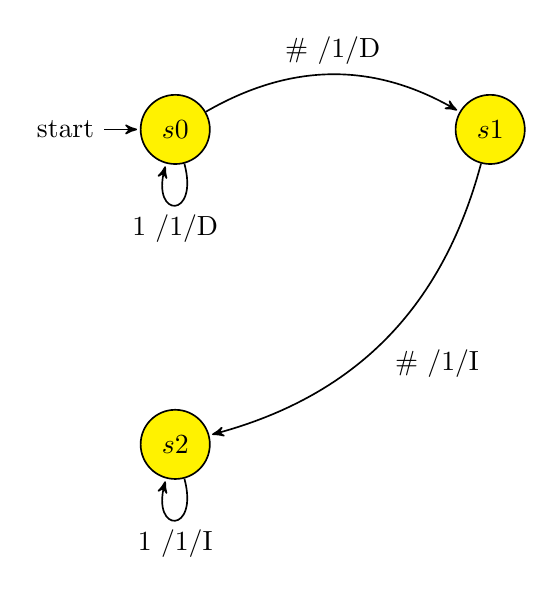
\begin{tikzpicture}[->,>=stealth',shorten >=1pt,auto,node distance=4cm,semithick]
\tikzstyle{every state}=[fill=yellow,text=black]

\node[state,initial] (s0) {$s0$};
\node[state,right of=s0] (s1) {$s1$};
\node[state,below of=s0] (s2) {$s2$};

\path
(s0) edge [loop below] node { 1 /1/D} (s0)
(s0) edge [bend left] node { \# /1/D} (s1)
(s1) edge [bend left] node { \# /1/I} (s2)
(s2) edge [loop below] node { 1 /1/I} (s2)
;
\end{tikzpicture}
\end{document}
